% Options for packages loaded elsewhere
% Options for packages loaded elsewhere
\PassOptionsToPackage{unicode}{hyperref}
\PassOptionsToPackage{hyphens}{url}
\PassOptionsToPackage{dvipsnames,svgnames,x11names}{xcolor}
%
\documentclass[
  letterpaper,
  DIV=11,
  numbers=noendperiod]{scrartcl}
\usepackage{xcolor}
\usepackage{amsmath,amssymb}
\setcounter{secnumdepth}{5}
\usepackage{iftex}
\ifPDFTeX
  \usepackage[T1]{fontenc}
  \usepackage[utf8]{inputenc}
  \usepackage{textcomp} % provide euro and other symbols
\else % if luatex or xetex
  \usepackage{unicode-math} % this also loads fontspec
  \defaultfontfeatures{Scale=MatchLowercase}
  \defaultfontfeatures[\rmfamily]{Ligatures=TeX,Scale=1}
\fi
\usepackage{lmodern}
\ifPDFTeX\else
  % xetex/luatex font selection
\fi
% Use upquote if available, for straight quotes in verbatim environments
\IfFileExists{upquote.sty}{\usepackage{upquote}}{}
\IfFileExists{microtype.sty}{% use microtype if available
  \usepackage[]{microtype}
  \UseMicrotypeSet[protrusion]{basicmath} % disable protrusion for tt fonts
}{}
\makeatletter
\@ifundefined{KOMAClassName}{% if non-KOMA class
  \IfFileExists{parskip.sty}{%
    \usepackage{parskip}
  }{% else
    \setlength{\parindent}{0pt}
    \setlength{\parskip}{6pt plus 2pt minus 1pt}}
}{% if KOMA class
  \KOMAoptions{parskip=half}}
\makeatother
% Make \paragraph and \subparagraph free-standing
\makeatletter
\ifx\paragraph\undefined\else
  \let\oldparagraph\paragraph
  \renewcommand{\paragraph}{
    \@ifstar
      \xxxParagraphStar
      \xxxParagraphNoStar
  }
  \newcommand{\xxxParagraphStar}[1]{\oldparagraph*{#1}\mbox{}}
  \newcommand{\xxxParagraphNoStar}[1]{\oldparagraph{#1}\mbox{}}
\fi
\ifx\subparagraph\undefined\else
  \let\oldsubparagraph\subparagraph
  \renewcommand{\subparagraph}{
    \@ifstar
      \xxxSubParagraphStar
      \xxxSubParagraphNoStar
  }
  \newcommand{\xxxSubParagraphStar}[1]{\oldsubparagraph*{#1}\mbox{}}
  \newcommand{\xxxSubParagraphNoStar}[1]{\oldsubparagraph{#1}\mbox{}}
\fi
\makeatother


\usepackage{longtable,booktabs,array}
\usepackage{calc} % for calculating minipage widths
% Correct order of tables after \paragraph or \subparagraph
\usepackage{etoolbox}
\makeatletter
\patchcmd\longtable{\par}{\if@noskipsec\mbox{}\fi\par}{}{}
\makeatother
% Allow footnotes in longtable head/foot
\IfFileExists{footnotehyper.sty}{\usepackage{footnotehyper}}{\usepackage{footnote}}
\makesavenoteenv{longtable}
\usepackage{graphicx}
\makeatletter
\newsavebox\pandoc@box
\newcommand*\pandocbounded[1]{% scales image to fit in text height/width
  \sbox\pandoc@box{#1}%
  \Gscale@div\@tempa{\textheight}{\dimexpr\ht\pandoc@box+\dp\pandoc@box\relax}%
  \Gscale@div\@tempb{\linewidth}{\wd\pandoc@box}%
  \ifdim\@tempb\p@<\@tempa\p@\let\@tempa\@tempb\fi% select the smaller of both
  \ifdim\@tempa\p@<\p@\scalebox{\@tempa}{\usebox\pandoc@box}%
  \else\usebox{\pandoc@box}%
  \fi%
}
% Set default figure placement to htbp
\def\fps@figure{htbp}
\makeatother





\setlength{\emergencystretch}{3em} % prevent overfull lines

\providecommand{\tightlist}{%
  \setlength{\itemsep}{0pt}\setlength{\parskip}{0pt}}



 
\usepackage[]{natbib}
\bibliographystyle{plainnat}


\usepackage{booktabs}
\usepackage{longtable}
\usepackage{array}
\usepackage{multirow}
\usepackage{wrapfig}
\usepackage{float}
\usepackage{colortbl}
\usepackage{pdflscape}
\usepackage{tabu}
\usepackage{threeparttable}
\usepackage{threeparttablex}
\usepackage[normalem]{ulem}
\usepackage{makecell}
\usepackage{xcolor}
\KOMAoption{captions}{tableheading}
\makeatletter
\@ifpackageloaded{caption}{}{\usepackage{caption}}
\AtBeginDocument{%
\ifdefined\contentsname
  \renewcommand*\contentsname{Table of contents}
\else
  \newcommand\contentsname{Table of contents}
\fi
\ifdefined\listfigurename
  \renewcommand*\listfigurename{List of Figures}
\else
  \newcommand\listfigurename{List of Figures}
\fi
\ifdefined\listtablename
  \renewcommand*\listtablename{List of Tables}
\else
  \newcommand\listtablename{List of Tables}
\fi
\ifdefined\figurename
  \renewcommand*\figurename{Figure}
\else
  \newcommand\figurename{Figure}
\fi
\ifdefined\tablename
  \renewcommand*\tablename{Table}
\else
  \newcommand\tablename{Table}
\fi
}
\@ifpackageloaded{float}{}{\usepackage{float}}
\floatstyle{ruled}
\@ifundefined{c@chapter}{\newfloat{codelisting}{h}{lop}}{\newfloat{codelisting}{h}{lop}[chapter]}
\floatname{codelisting}{Listing}
\newcommand*\listoflistings{\listof{codelisting}{List of Listings}}
\makeatother
\makeatletter
\makeatother
\makeatletter
\@ifpackageloaded{caption}{}{\usepackage{caption}}
\@ifpackageloaded{subcaption}{}{\usepackage{subcaption}}
\makeatother
\usepackage{bookmark}
\IfFileExists{xurl.sty}{\usepackage{xurl}}{} % add URL line breaks if available
\urlstyle{same}
\hypersetup{
  pdftitle={Moreton Bay Seagrass Resilience Modelling},
  pdfauthor={Michael Dumelle (Dumelle Consulting); Erin E. Peterson (EP Consulting)},
  colorlinks=true,
  linkcolor={blue},
  filecolor={Maroon},
  citecolor={Blue},
  urlcolor={Blue},
  pdfcreator={LaTeX via pandoc}}


\title{Moreton Bay Seagrass Resilience Modelling}
\usepackage{etoolbox}
\makeatletter
\providecommand{\subtitle}[1]{% add subtitle to \maketitle
  \apptocmd{\@title}{\par {\large #1 \par}}{}{}
}
\makeatother
\subtitle{DRFA 21/22 Biodiversity Conservation Marine Final Report
Project}
\author{Michael Dumelle (Dumelle Consulting) \and Erin E. Peterson (EP
Consulting)}
\date{2026-05-11}
\begin{document}
\maketitle

\renewcommand*\contentsname{Table of contents}
{
\hypersetup{linkcolor=}
\setcounter{tocdepth}{3}
\tableofcontents
}

\section{Introduction}\label{introduction}

Over the past few decades, various scientific studies have informed our
current understanding of trends, behaviors, and flood responses of
seagrass cover in Moreton Bay
\citep{abal1996seagrass, udy1997growth, samper2016organic, ovsyanikova2026spatial}
as well as Australia more widely
\citep{kilminster2015unravelling, gilby2018seagrass, o2018seagrass}.
Remote sensing has offered new capabilities for seagrass cover mapping
\citep{roelfsema2009integrated}, while innovative statistical approaches
have offered novel methods for studying resilience at site-specific
scales \citep{gilby2023drivers}. Our work adds to this body of
literature by applying spatially explicit statistical models
\citep{cressie1993statistics} to study the drivers, resilience, and
recovery of total percent seagrass cover in Moreton Bay and Wide Bay
\citep{dumelle2026wide}. Specifically, we provide and contextualize
answers to three specific research questions, applicable to Moreton Bay:

\begin{enumerate}
\def\labelenumi{\arabic{enumi}.}
\tightlist
\item
  Can we identify water quality covariates that act as triggers for
  seagrass cover management responses? Are these triggers different
  based on whether they result from a specific event (e.g., flood) or
  ambient conditions?
\item
  Did seagrass cover improve after the flood event(s)? If so, how and
  where?
\item
  Can we identify site-specific resilience indicators, which describe
  where recovery is likely to be enhanced or impeded? If so, what
  factors contribute to seagrass resilience?
\end{enumerate}

\section{Seagrass Cover Model}\label{seagrass-cover-model}

\subsection{Methods}\label{methods}

\subsubsection{Data}\label{data}

The seagrass cover dataset was provided by Science Under Sail Australia
(SUSA; https://www.scienceundersail.com.au/). It included 7657
observations across three financial years (2020-2021, 2022-2023, and
2023-2024), where water quality and geographic covariates were also
available. Of the 7657 observations, 1995 were collected in 2020-2021
(pre-flood), 3329 in 2022-2023 (1-year post-flood), and 2333 in
2023-2024 (2-years post-flood) (Table~\ref{tbl-n_fy_mb}). There were six
seagrass species found in the dataset: \emph{Halophila decipiens} (HD),
\emph{Halophila spinulosa} (HS), \emph{Halophila ovalis} (HO),
\emph{Halodule uninervis} / \emph{Zostera muelleri} (ZMHU),
\emph{Syringodium isoetifolium} (SI) and \emph{Cymodocea serrulata}
(CS).

\begin{table}

\caption{\label{tbl-n_fy_mb}The sample size and percent of total sample
size for total percent seagrass cover observations in Moreton Bay, by
financial year.}

\centering{

\centering
\begin{tabular}{lrl}
  \toprule
Financial Year & Sample Size & Percent of Total \\ 
  \midrule
2020-2021 & 1995.00 & 26.1\% \\ 
  2022-2023 & 3329.00 & 43.5\% \\ 
  2023-2024 & 2333.00 & 30.5\% \\ 
  Total & 7657.00 & 100.0\% \\ 
   \bottomrule
\end{tabular}

}

\end{table}%

Seagrass cover is a percentage ranging from 0 (no seagrass) to 100
(complete seagrass cover). Total cover tends to be highest near the
eastern shoreline of the Bay and lowest in the middle
(Figure~\ref{fig-cover_fy_mb}). Note that 2022-2023 (post-flood) had the
the largest number of seagrass cover samples, as well as the only
samples collected in the middle of the Bay.

\begin{figure}

\centering{

\pandocbounded{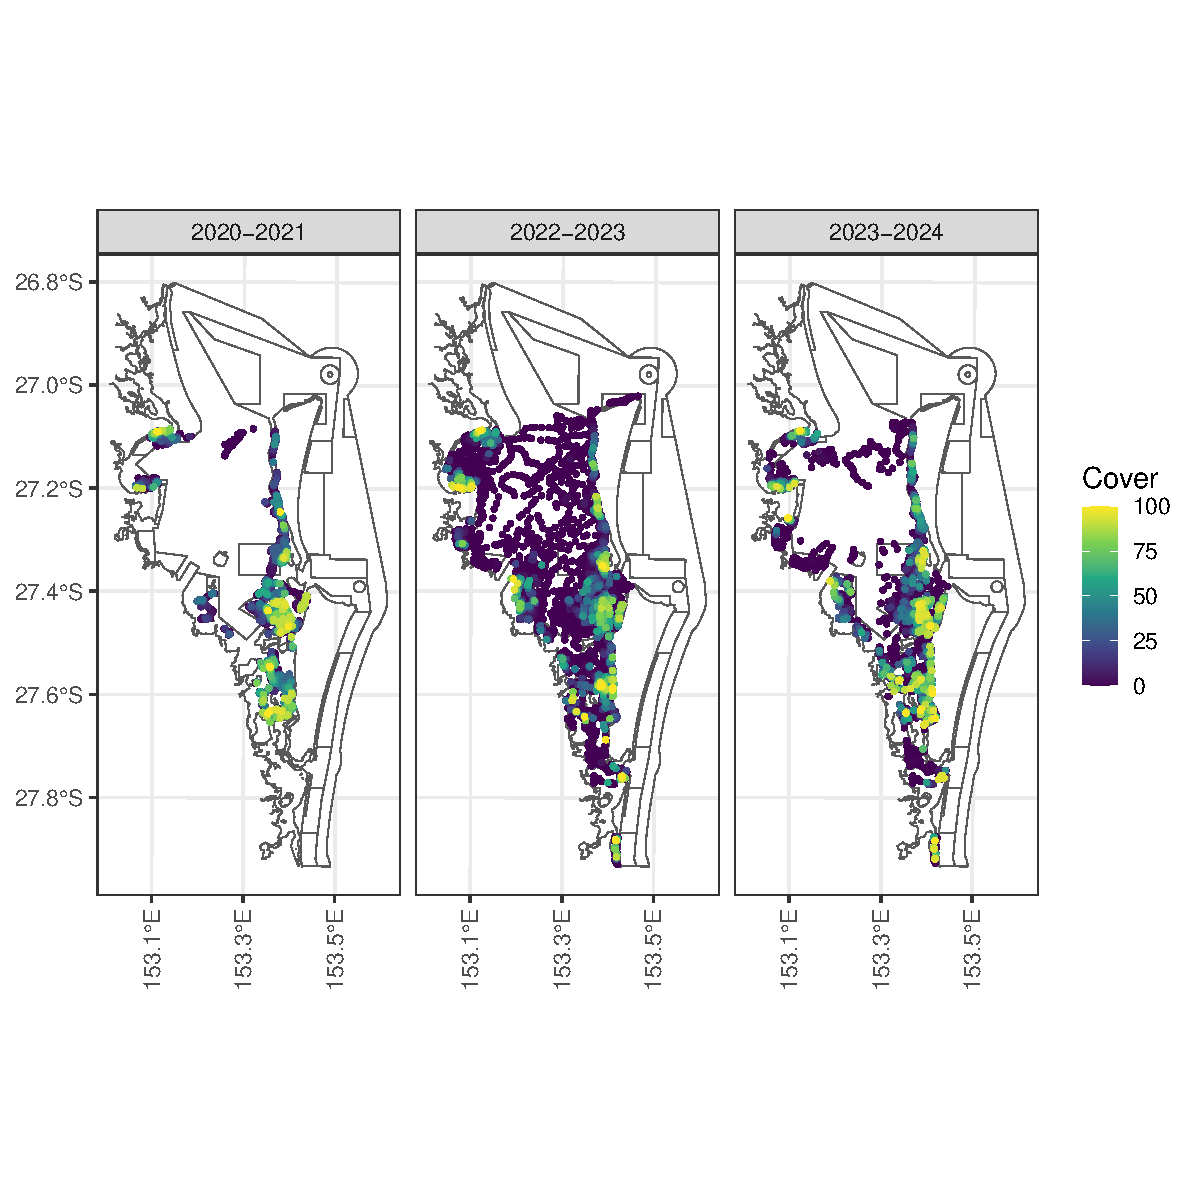
\includegraphics[keepaspectratio]{MBreport_files/figure-pdf/fig-cover_fy_mb-1.pdf}}

}

\caption{\label{fig-cover_fy_mb}Total percent seagrass cover in Moreton
Bay by financial year.}

\end{figure}%

EcoFutures Consulting used eReefs data \citep{steven2019ereefs} to
generate a broad suite of ambient and flood-related turbidity, salinity,
and temperature variables at biologically and ecologically relevant
temporal windows (Table~\ref{tbl-wq_vars_mb}). Ambient water quality
variables were based on the mean, minimum, and maximum values for three
periods: 7, 30, and 90 days prior to sampling. Ambient variables were
also calculated representing the frequency of days water quality
thresholds were exceeded (above or below) and the maximum spell (i.e.,
duration) of days those thresholds were continuously exceeded during the
time periods. Similar water quality variables representing flood-event
conditions were also calculated for a 30-day flood period.

\begin{table}

\caption{\label{tbl-wq_vars_mb}Moreton Bay water quality variables
considered in the exploratory analyses, including the variable name and
measurement unit (in parentheses), the type of water-quality variable
(Ambient, Flood), the time period in days, statistic calculated, and the
threshold value used (if any).}

\centering{

\centering
\begin{tabular}{lllll}
  \toprule
Variable & Type & Period & Statistic & Threshold \\ 
  \midrule
Turbidity (NTU) & Ambient & 30, 7, 90 & Mean &  \\ 
  Turbidity (NTU) & Ambient & 30, 7, 90 & Frequency & $>$ 3 \\ 
  Turbidity (NTU) & Ambient & 30, 7, 90 & Frequency & $>$ 5 \\ 
  Turbidity (NTU) & Ambient & 30, 7, 90 & Frequency & $>$ 6 \\ 
  Salinity (PSU) & Ambient & 30, 7, 90 & Frequency & $<$ 20 \\ 
  Salinity (PSU) & Ambient & 30, 7, 90 & Frequency & $<$ 25 \\ 
  Salinity (PSU) & Ambient & 30, 7, 90 & Frequency & $<$ 30 \\ 
  Temperature (deg C) & Ambient & 30, 7, 90 & Mean &  \\ 
  Turbidity (NTU) & Flood & 30 & Mean &  \\ 
  Turbidity (NTU) & Flood & 30 & Max &  \\ 
  Turbidity (NTU) & Flood & 30 & Frequency & $>$ 3 \\ 
  Turbidity (NTU) & Flood & 30 & Frequency & $>$ 5 \\ 
  Turbidity (NTU) & Flood & 30 & Frequency & $>$ 6 \\ 
  Turbidity (NTU) & Flood & 30 & Duration & $>$ 3 \\ 
  Turbidity (NTU) & Flood & 30 & Duration & $>$ 5 \\ 
  Turbidity (NTU) & Flood & 30 & Duration & $>$ 6 \\ 
  Salinity (PSU) & Flood & 30 & Min &  \\ 
  Salinity (PSU) & Flood & 30 & Mean &  \\ 
  Salinity (PSU) & Flood & 30 & Frequency & $<$ 20 \\ 
  Salinity (PSU) & Flood & 30 & Frequency & $<$ 25 \\ 
  Salinity (PSU) & Flood & 30 & Frequency & $<$ 30 \\ 
  Salinity (PSU) & Flood & 30 & Duration & $<$ 20 \\ 
  Salinity (PSU) & Flood & 30 & Duration & $<$ 25 \\ 
  Salinity (PSU) & Flood & 30 & Duration & $<$ 30 \\ 
   \bottomrule
\end{tabular}

}

\end{table}%

Additional covariates were provided by EcoFutures Consulting
representing geographic features, proximity to rivers, and depth, as
well as the years since the flood and seagrass growing season. These
variables have the following structure:

\begin{itemize}
\tightlist
\item
  Sediment Type includes six categorical levels: Sand, Sandy Mud, Muddy
  Sand, Mud, Rock, and Other.
\item
  Tidal Range has three categorical levels: Shallow Subtidal,
  Intertidal, and Deep Subtidal.
\item
  Years Since Flood is numeric ranging from zero (pre flood) to 1.93
  years post-flood (February, 2024).
\item
  Nearest River includes six categorical levels: Brisbane River,
  Caboolture River, Logan River, Ningi Creek, Pimpama Coomera and Nerang
  Rivers, and Pine River.
\item
  Distance to (Nearest River) Outlet is numeric and ranges from 0.24 to
  34.97 kilometers.
\item
  Growing Season is a categorical variable with two levels: Growing
  (September - December) and Not Growing (January - August).
\item
  EHMP subzone has eleven categorical levels: Bramble Bay, Broadwater,
  Central Bay, Deception Bay, Eastern Banks, Moreton Bay Open Coastal
  Waters, North-Eastern Moreton Bay, Northern Banks Open Coastal Waters,
  South-Eastern Moreton Bay, Southern Bay, and Waterloo Bay
  (Figure~\ref{fig-ehmp_subzone}).
\end{itemize}

\begin{figure}

\centering{

\pandocbounded{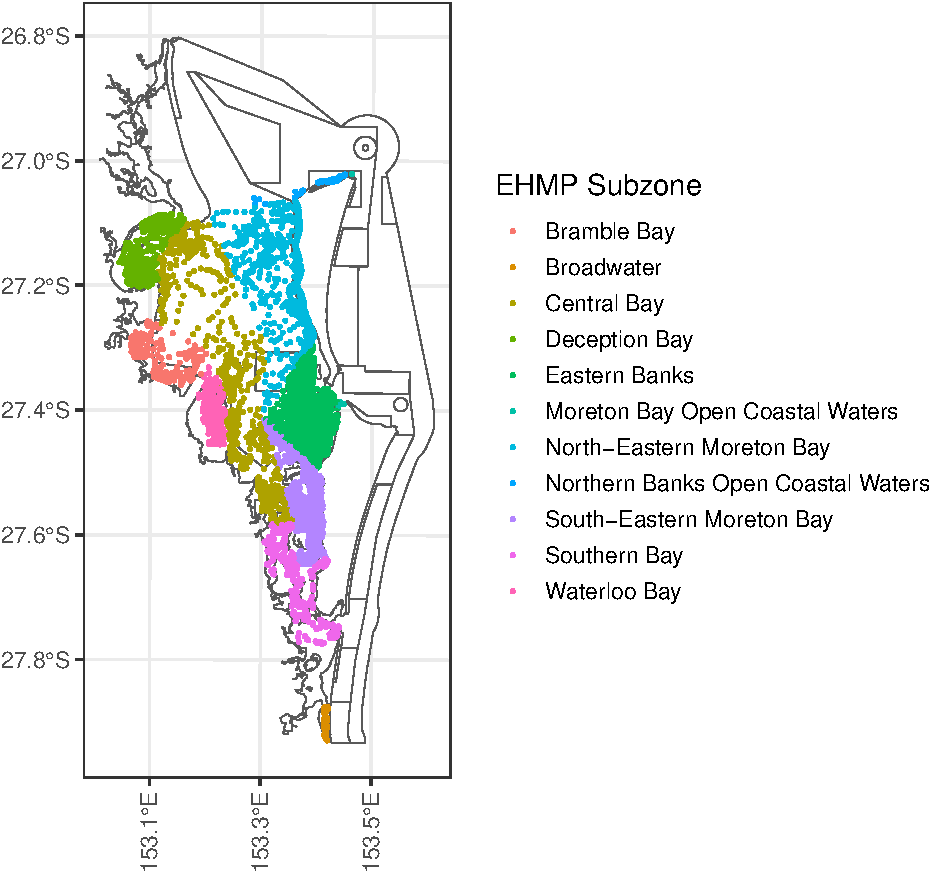
\includegraphics[keepaspectratio]{MBreport_files/figure-pdf/fig-ehmp_subzone-1.pdf}}

}

\caption{\label{fig-ehmp_subzone}Observations and their EHMP Subzones in
Moreton Bay.}

\end{figure}%

\subsubsection{Exploratory Analyses}\label{exploratory-analyses}

Extensive exploratory analyses were undertaken to 1) understand the data
structure, 2) visualize spatial and temporal patterns in the data, 3)
identify outliers/errors, 4) examine correlations between potential
covariates and the seagrass cover, as well as multicollinearity among
covariates, 5) compare the fit of various models, and 6) evaluate model
assumptions.

Results revealed substantial collinearity among ambient and
flood-related water-quality variables, as expected given their nested
temporal windows and threshold values. We retained only one variable
from each correlated group and prioritized sediment type, tidal range,
turbidity, temperature, and time since flood when making these
decisions. We also removed other variables showing no meaningful
association with seagrass cover or where the relationship lacked
biological plausibility. This included all of the salinity variables,
which had little variability and did not exhibit strong relationships
with seagrass cover. Geographic variables exhibited less collinearity
than water quality variables; however, we removed the distance to the
nearest river outlet and the nearest river variables due to weak
associations with seagrass cover after accounting for other model
covariates. Growing season was excluded because a simple monthly proxy
inadequately captures seasonal seagrass growth dynamics.

The final set of potential covariates considered in the modelling
included mean turbidity in the 90 days prior to sampling, mean turbidity
during the flood event, mean temperature in the 90 days prior to
sampling, sediment type, tidal range, years since flood, and EHMP
subzone.

\subsubsection{Statistical Modeling}\label{sec-mb_model}

We considered multiple modeling approaches in this study, which each
accounted for the data distribution, nonlinear relationships between
seagrass cover and covariates, and spatial dependence inherent in
biological data collected through space and time to different degrees
(Appendix 1). We used the full set of potential covariates to fit a
nonspatial linear model, spatial linear model (i.e., spatial model),
spatial beta regression model, spatial gamma regression model, and a
random forest model, comparing the model fit of each.

There were several reasons for fitting these initial models. The
nonspatial linear model provided a useful baseline to compare the
spatial linear model against, elucidating the impact of spatial
dependence on model fit. The spatial beta regression model is a
generalized linear model used to characterize bounded proportional data
ranging between zero and one. To adhere to this restriction, total
seagrass cover was 1) scaled to a proportion and 2) if exactly zero or
one, set to 0.01 or 0.99, respectively. The spatial gamma regression
model is a generalized linear model used to characterize skewed positive
data. To adhere to this restriction, a value of 0.01 was added to
seagrass cover observations that were equal to zero. Finally, the random
forest model provided a useful assessment of a machine learning
approach, which requires fewer distributional assumptions than the
aforementioned statistical approaches and more naturally describes
nonlinear relationships between variables (Appendix 1). We also
characterized random forest effects using partial dependence plots
\citep{greenwell2017pdp}, which isolate the marginal contribution of a
variable while holding other variables at their observed values.
Out-of-sample predictions were generated for the four statistical models
using leave-one-out cxross validation, while out-of-bag validation was
used for the random forest model. These out-of-sample predictions were
then used to calculate the mean bias (MBias) and
root-mean-square-prediction error (RMSPE) for each model.

The results of this initial model comparison showed that the spatial
linear model had the lowest RMSPE, followed by the random forest,
generalized linear models, and the nonspatial linear model
(Table~\ref{tbl-mb_cv}). Mean bias (MBias) tended to be small relative
to root-mean-squared-prediction error (RMSPE). The nonspatial and
spatial linear models also had much lower mean bias values than the
random forest model, while the two generalized linear models produced
unacceptably biased predictions. Nevertheless, all five approaches
identified similar relationships between seagrass cover and the
covariates, in the directions expected. Random forest partial dependence
plots \citep{greenwell2017pdp} suggested that linear effects of the
model variables were generally reasonable. We chose to use a spatial
linear modeling framework for the Moreton Bay seagrass model based on
these results and the ease of interpretability.

\begin{table}

\caption{\label{tbl-mb_cv}Moreton Bay out of sample prediction metrics
for the five modeling approaches, including mean bias (MBias) and root
mean square prediction error (RMSPE).}

\centering{

\centering
\begin{tabular}{lrr}
  \toprule
Approach & MBias & RMSPE \\ 
  \midrule
Spatial Linear Model & -0.016 & 18.415 \\ 
  Random Forest & -0.111 & 18.838 \\ 
  Spatial GLM - Beta & -2.759 & 19.599 \\ 
  Spatial GLM - Gamma & 5.424 & 20.066 \\ 
  Linear Model & 0.001 & 22.536 \\ 
   \bottomrule
\end{tabular}

}

\end{table}%

\begin{figure}

\centering{

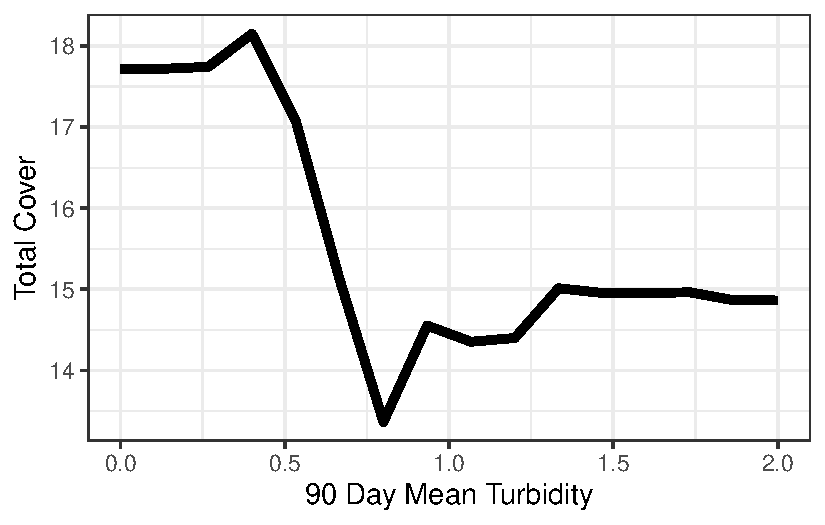
\includegraphics[width=0.5\linewidth,height=\textheight,keepaspectratio]{MBreport_files/figure-pdf/fig-rf_turb-1.pdf}

}

\caption{\label{fig-rf_turb}Random forest partial dependence for
seagrass cover as a function of mean turbidity in the 90 days prior to
sampling.}

\end{figure}%

A suite of spatial linear models (Appendix 1, Equation~\ref{eq-splm1}),
with exponential spatial covariance functions and a random effect for
EHMP subzone, were fit using the \texttt{splm()} function in
\texttt{spmodel} \citet{dumelle2023spmodel}. Parameters were estimated
using restricted maximum likelihood and models primarily compared using
leave-one-out cross validation; though AIC or BIC could also be used if
parameters were estimated using maximum likelihood. In addition, the
relationships between seagrass cover and covariates needed to be
plausible.

The final total seagrass cover model for Moreton Bay included the
following covariates: tidal range, sediment type, 90-day mean
temperature (prior to sampling), 90 day turbidity (prior to sampling),
and mean turbidity during the flood period scaled by time since the
flood squared (Table~\ref{tbl-mb_tc_splm_vars}). Mean turbidity during
the flood period was scaled so that its effect decays with time since
the flood. Intuitively, this means that as the time since the flood
increases, the impact of turbidity during the flood event decreases. We
also considered scaling by time since flood (not squared), which
produced similar results.

\begin{table}

\caption{\label{tbl-mb_tc_splm_vars}Covariates in the final Moreton Bay
seagrass cover model, their type (numeric or categorical), and if
categorical, the number of unique levels.}

\centering{

\centering
\begin{tabular}{lll}
  \toprule
Variable & Type & No. Levels \\ 
  \midrule
90 Day Temperature & Numeric & NA \\ 
  90 Day Turbidity & Numeric & NA \\ 
  Mean Flood Turbidity/Years Since Flood\verb|^|2 & Numeric & NA \\ 
  Sediment Type & Categorical & 6 \\ 
  Tidal Range & Categorical & 3 \\ 
   \bottomrule
\end{tabular}

}

\end{table}%

\begin{table}

\caption{\label{tbl-mb-fixed}Fixed effects table of covariates in the
Moreton Bay water quality and geographic model.}

\centering{

\centering
\begin{tabular}{lrrr}
  \toprule
Term & Estimate & z & p.value \\ 
  \midrule
Intercept (Mud/Deep Subtidal) & -13.683 & -2.312 & 0.021 \\ 
  Muddy Sand & 4.825 & 5.674 & 0.000 \\ 
  Other & 11.296 & 1.188 & 0.235 \\ 
  Rock & -8.661 & -5.328 & 0.000 \\ 
  Sand & -0.095 & -0.098 & 0.922 \\ 
  Sandy Mud & 3.492 & 4.032 & 0.000 \\ 
  Intertidal & 22.014 & 24.671 & 0.000 \\ 
  Shallow Subtidal & 11.633 & 16.414 & 0.000 \\ 
  90 Day Temperature & 0.876 & 4.119 & 0.000 \\ 
  90 Day Turbidity & -7.181 & -2.802 & 0.005 \\ 
  Mean Flood Turbidity/Years Since Flood\verb|^|2 & -2.056 & -3.459 & 0.001 \\ 
   \bottomrule
\end{tabular}

}

\end{table}%

Table~\ref{tbl-mb-fixed} shows the fixed effects table from the fitted
model. The reference group is the muddy and deep subtidal group, and the
remaining sediment type and tidal range terms represent deviations from
these baselines. For the numeric variables, all had small \(p\)-values
(\(p\)-value \(<\) 0.01). While we can assess the overall significance
of the numeric variables Table~\ref{tbl-mb-fixed}, we must perform an
analysis of variance (ANOVA) to assess the overall significance of
variables with many levels. Table~\ref{tbl-mb-covariates} shows these
ANOVA results for the sediment type and tidal range variables, which had
small \(p\)-values (\(p\)-value \(<\) 0.01). Together, these results
indicate all variables had a significant relationship with total
seagrass cover. Here are some relevant takeaways from the model fit:

\begin{itemize}
\tightlist
\item
  Tidal Range: The estimated (marginal) average total cover is largest
  in the intertidal (26.89\%), followed by shallow subtidal (16.51\%)
  and deep subtidal (4.88\%).
\item
  Sediment Type: The estimated (marginal) average total cover is largest
  in the other category (25.6\%), followed by muddy sand (19.1\%), sandy
  mud (17.8\%), mud (14.3\%), sand (14.2\%), and rock (5.62\%). The
  other category results should be interpreted with caution, as there
  are only four observations.
\item
  90 Day Temperature: A one-degree (C) increase in 90-day water
  temperature prior to sampling is associated with a decrease in average
  seagrass cover by 0.88\%.
\item
  Mean Flood Turbidity/(Years Since Flood)\(^2\): A one-unit increase in
  mean turbidity during the flood is associated with a decrease in
  average seagrass cover of 2.05\%/(Years Since Flood)\(^2\)
  (Figure~\ref{fig-mb_turb_90d_fld}).
\item
  90 Day Turbidity: A one-unit increase in 90-day turbidity (prior to
  sampling) is associated with a decrease in average seagrass cover by
  7.18\% (Figure~\ref{fig-mb_turb_90d_fld}).
\end{itemize}

\begin{table}

\caption{\label{tbl-mb-covariates}ANOVA table of covariates for the
categorical variables in the Moreton Bay water quality and geographic
model.}

\centering{

\centering
\begin{tabular}{lrrr}
  \toprule
Effects & df & Chi-sq & p.value \\ 
  \midrule
Tidal Range &    2 & 608.900 & 0.000 \\ 
  Sediment Type &    5 & 113.720 & 0.000 \\ 
   \bottomrule
\end{tabular}

}

\end{table}%

\begin{figure}

\centering{

\pandocbounded{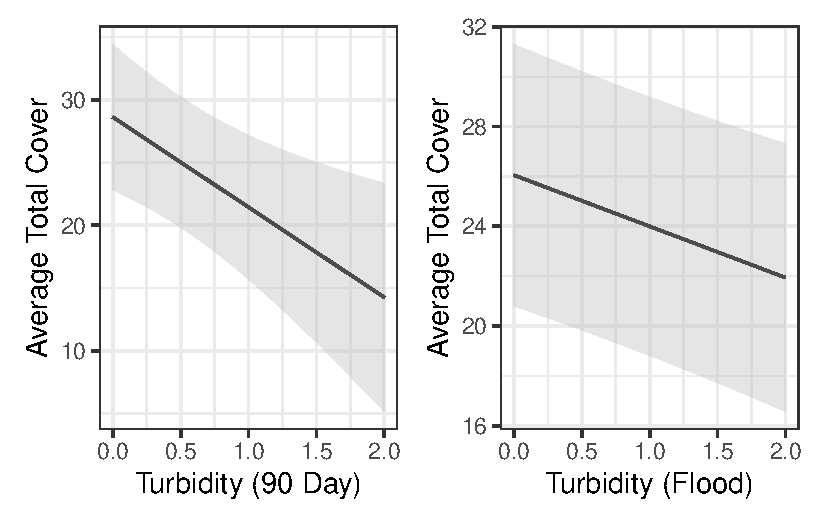
\includegraphics[keepaspectratio]{MBreport_files/figure-pdf/fig-mb_turb_90d_fld-1.pdf}}

}

\caption{\label{fig-mb_turb_90d_fld}Average total seagrass percent cover
as a function of 90-day mean turbidity (left) and flood turbidity
(right). Estimates (and confidence intervals) were evaluated at one year
post flood, at the means of all other numeric variables, and for the
intertidal range and sand sediment types.}

\end{figure}%

We examined model diagnostics to better understand the overall model
fit. First, we partitioned the model into different components of
variability (Table~\ref{tbl-mb_varcomp}) and found that 11.2\% is
attributable to the covariates (a quantity sometimes referred to as the
Pseudo R-squared), 31.6\% to the spatial random error, 7.3\% to the EHMP
subzone, and the remaining variability is independent random error.
Second, we examined the decay behaviour of spatial autocorrelation. The
estimated exponential spatial range (\(\phi\)) is 745.5 meters, which
suggests two total seagrass cover observations are approximately
(spatially) uncorrelated at a distance of \(3\phi \approx 2\)km, or two
kilometers. Third, we analyzed the standardized model residuals, which
have been decorrelated, to assess model assumptions and identify
influential observations that had a sizable impact on model fit.
Generally, the standardized residuals are centered around zero, though
there is a slight right skew suggesting some observed total cover values
are larger than expected (according to the model). Observations are
referred to as ``influential'' if they highly influence model fit.
Influence is often assessed using a Cook's distance threshold value of
one \citep{cook1982residuals}. No observations exceed this threshold.

\begin{table}

\caption{\label{tbl-mb_varcomp}Variance components in the Moreton Bay
seagrass model.}

\centering{

\centering
\begin{tabular}{llr}
  \toprule
Variance Component & Percent (of Total Variability) & Parameter Value \\ 
  \midrule
Covariates & 11.2\% &  \\ 
  Spatial Effect & 31.6\% & 182.1 \\ 
  Independent Error & 49.9\% & 287.5 \\ 
  EHMP Subzone & 7.3\% & 745.5 \\ 
   \bottomrule
\end{tabular}

}

\end{table}%

\subsubsection{Block Kriging}\label{block-kriging}

A tremendous benefit of using the spatial linear model is that block
Kriging \citep{ver2002sampling, cressie2006block} can be used to predict
the mean total seagrass cover bay-wide for any combination of covariates
and geographic regions, even if these variables were not directly used
in the model (see Appendix 1 for additional details). Block Kriging was
undertaken, by financial year, for EHMP subzone, Marine Park zone, tidal
range and for the whole of Moreton Bay.

Figure~\ref{fig-bk_mb_ehmp} and Figure~\ref{fig-bk_mb_zone} show there
are several EHMP subzones and Marine Park zones that have recovered to
pre-flood levels (e.g., Deception Bay, Marine National Park Zone), while
others have not (e.g., Southern Bay, General Use Zone). When we examine
recovery by tidal range (Figure~\ref{fig-bk_mb_tidal}), we see that
seagrass cover is recovering across all tidal ranges. When we examine
recovery for the whole of Moreton Bay (Figure~\ref{fig-bk_mb_all}), the
model suggests that seagrass cover has improved since the 2022 flood.

\begin{figure}

\centering{

\pandocbounded{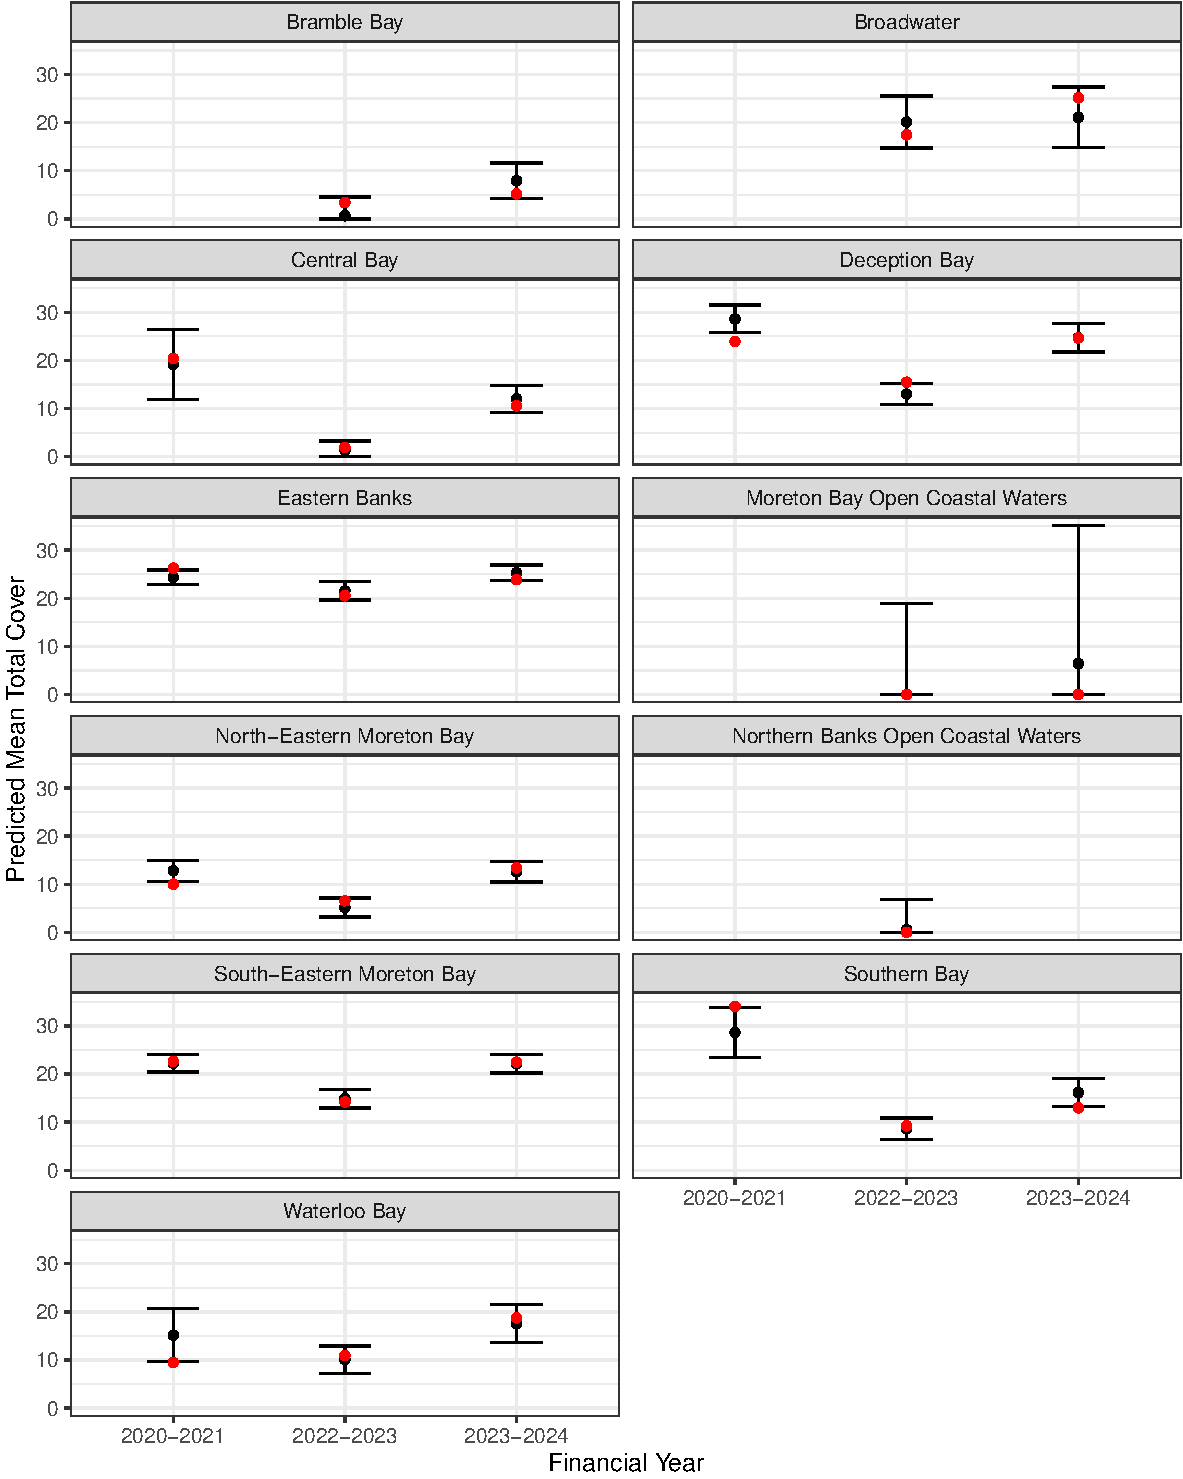
\includegraphics[keepaspectratio]{MBreport_files/figure-pdf/fig-bk_mb_ehmp-1.pdf}}

}

\caption{\label{fig-bk_mb_ehmp}Average total cover predictions by EHMP
subzone. Red dots indicate the mean from the raw data. Black dots
indicate the predicted mean in the region alongside a prediction
interval.}

\end{figure}%

\begin{figure}

\centering{

\pandocbounded{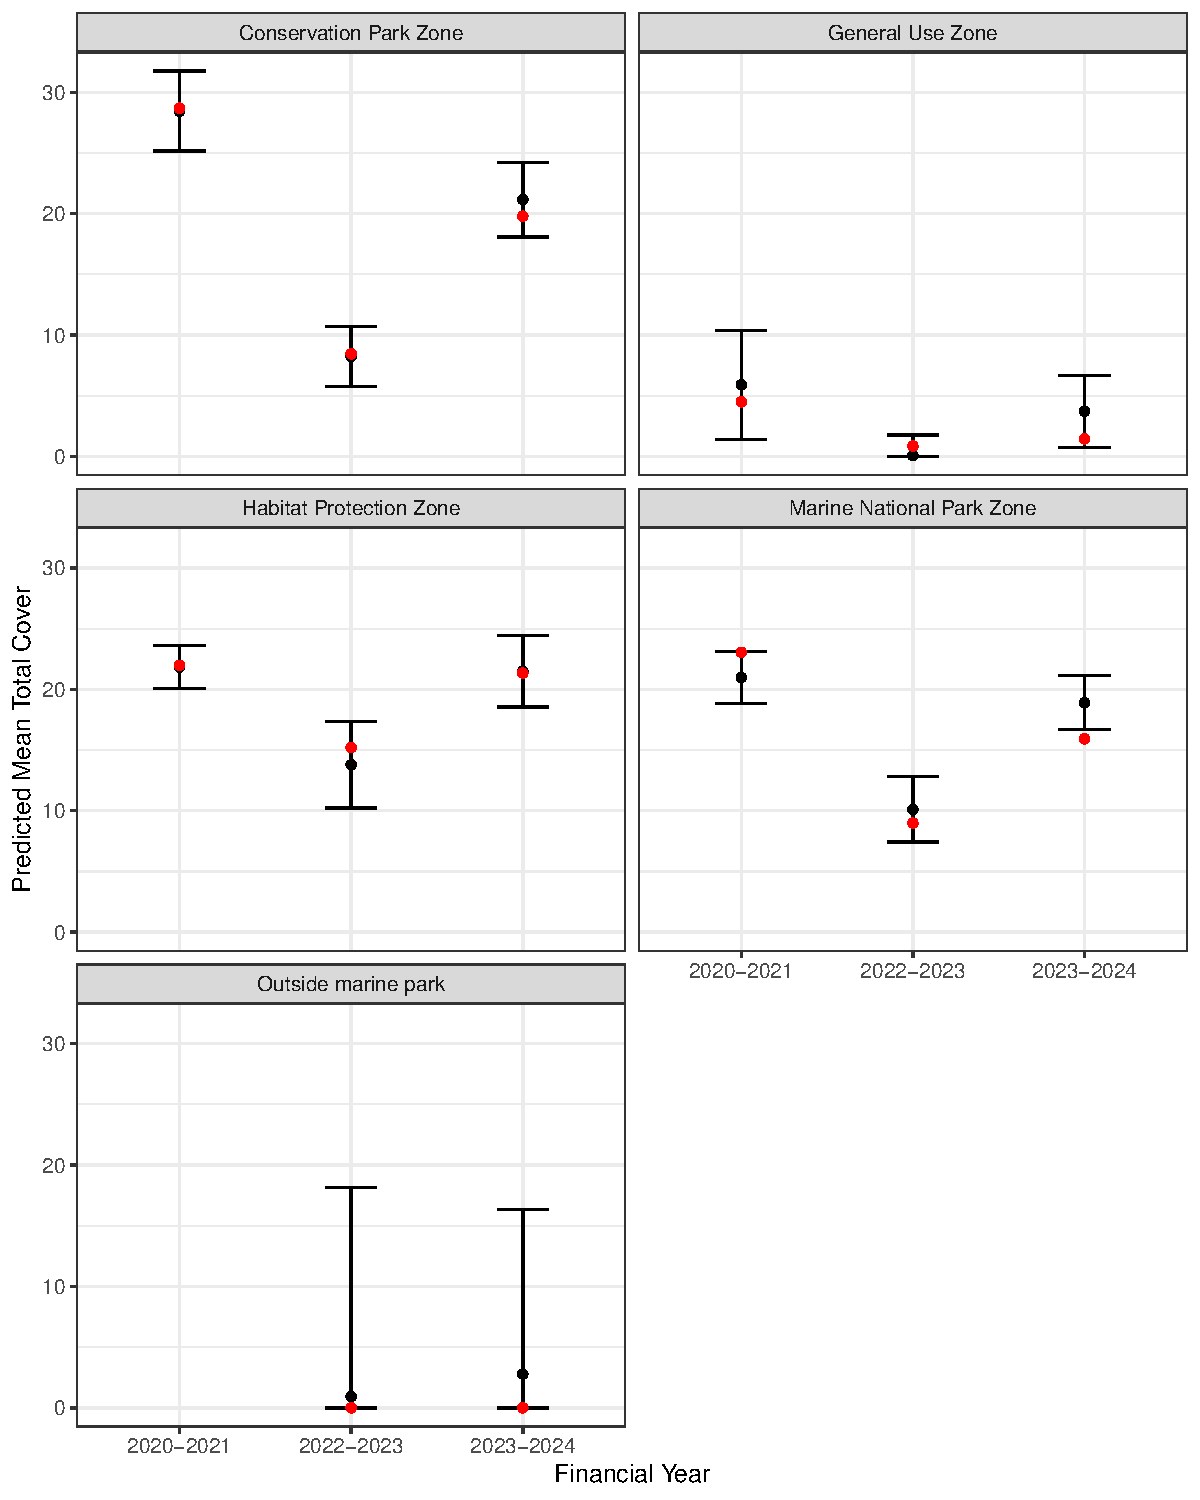
\includegraphics[keepaspectratio]{MBreport_files/figure-pdf/fig-bk_mb_zone-1.pdf}}

}

\caption{\label{fig-bk_mb_zone}Average total seagrass cover predictions
by conservation zone. Red dots indicate the mean from the raw data.
Black dots indicate the predicted mean in the region alongside a
prediction interval.}

\end{figure}%

\begin{figure}

\centering{

\pandocbounded{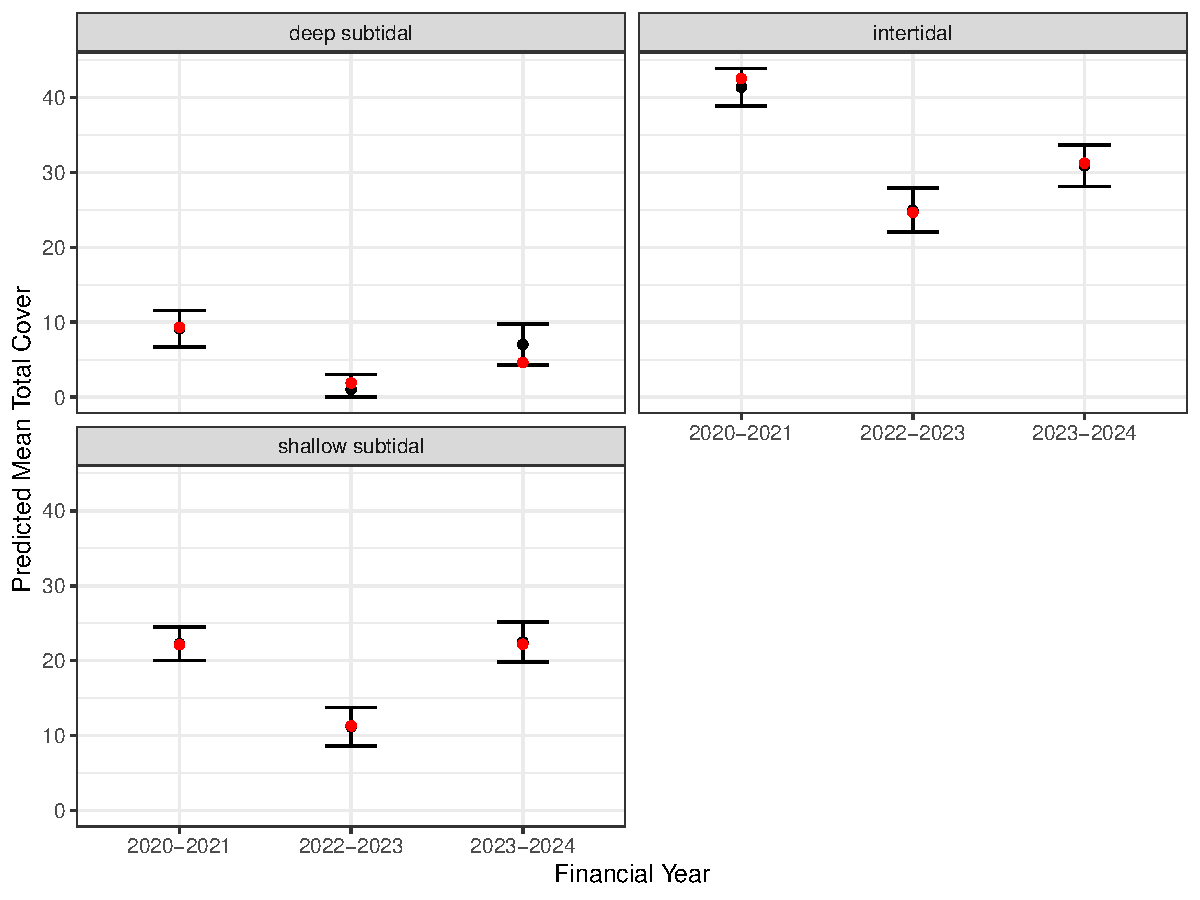
\includegraphics[keepaspectratio]{MBreport_files/figure-pdf/fig-bk_mb_tidal-1.pdf}}

}

\caption{\label{fig-bk_mb_tidal}Average total seagrass cover predictions
by tidal range. Red dots indicate the mean from the raw data. Black dots
indicate the predicted mean in the region alongside a prediction
interval.}

\end{figure}%

\begin{figure}

\centering{

\pandocbounded{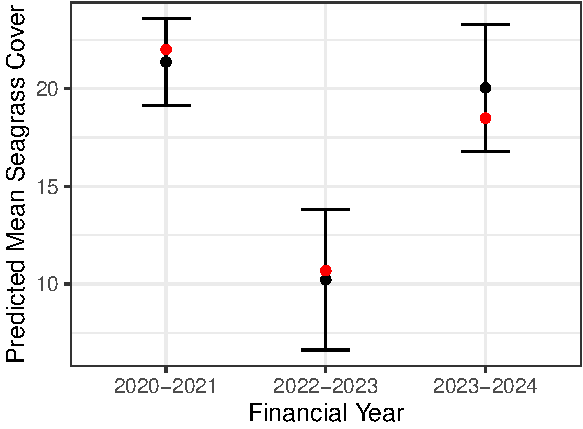
\includegraphics[keepaspectratio]{MBreport_files/figure-pdf/fig-bk_mb_all-1.pdf}}

}

\caption{\label{fig-bk_mb_all}Average total seagrass cover predictions
in Moreton Bay. Red dots indicate the mean from the raw data. Black dots
indicate the predicted mean in the region alongside a prediction
interval.}

\end{figure}%

\clearpage

\section{Resilience Model}\label{sec-mb_resilience}

The seagrass cover model quantifies bay-wide effects of influential
drivers on seagrass cover and enables assessment of recovery
trajectories at management-relevant scales. However, it does not
quantify site-specific resilience. \citet{gilby2023drivers} propose
identifying hotspots (i.e., brightspots, sites performing better than
expected) and coldspots (sites performing worse than expected) based on
model residuals exceeding confidence interval bounds. They argue that
hotspots and coldspots offer significant utility for understanding
drivers of site-specific resilience and informing management decisions.
\citet{gilby2023drivers} primarily focused on specific hotspots, linking
environmental variables to those sites. We build on that work by using
the seagrass model residuals as a proxy for site-specific resilience,
and then characterizing the most important drivers of that resilience.

\subsection{Methods}\label{methods-1}

\subsubsection{Data}\label{data-1}

We used the raw seagrass model residuals (Figure~\ref{fig-resid_fy_mb})
as a the response variable in a second spatial linear model used to
study site-specific resilience in Moreton Bay. Model covariates included
variables describing seagrass richness and dominant species, and
bathymetry, as well as distance to the nearest coral, seagrass,
mangrove, or gastropod habitat, and the total area in msq of coral,
seagrass, mangrove, or gastropod habitat within 500 m of the observation
point (Table~\ref{tbl-res_vars_mb}). EHMP subzone was again included as
a random effect. Because we were interested in hypothesis testing rather
than parsimony, we included all potential covariates as fixed effects in
the model. Potential covariates have the following structure:

\begin{itemize}
\tightlist
\item
  Coral Habitat Total Area is numeric from 0 msq to 616,180 meters
  squared (msq).
\item
  Seagrass Habitat Total Areais numeric from 0 msq to 773,161 msq.
\item
  Mangrove Habitat Total Area is numeric from 0 msq to 561,317 msq.
\item
  Gastropod Habitat Total Area is numeric from 0 msq to 114,795 msq.
\item
  Distance to Coral Habitat is numeric from 0 m to 35,387 m.
\item
  Distance to Seagrass Habitat is numeric from 0 m to 11,382 m.
\item
  Distance to Mangrove Habitat is numeric from 0 m to 27,617 m.
\item
  Distance to Gastropod Habitat is numeric from 0 m to 32,034 m.
\item
  Habitat Count is numeric (integer) from 0 to 4 unique habitats (coral,
  seagrass, mangrove, gastropod).
\item
  Species Richness is numeric (integer) from 0 to 4 unique species
  (possible species: ``Absent'', ``CS'', ``HD'', ``HO'', ``HS'', ``SI'',
  and ``ZMHU'').
\item
  Dominant Species represents the dominant seagrass species and has
  seven levels: ``Absent'', ``CS'', ``HD'', ``HO'', ``HS'', ``SI'', and
  ``ZMHU''.
\item
  Bathymetry Mean Depth is the GBR mean depth within 500 m of the
  seagrass observation point, excluding terrestrial areas, and is
  numeric from -35.95 m to 0.79 m.
\item
  Bathymetry Mean Curvature is the GBR mean curvature within 500 m of
  the seagrass observation point, excluding terrestrial areas, and is
  numeric from -0.002 degrees to 0.0001 degrees.
\item
  Bathymetry Mean Slope is the GBR mean slope within 500 m of the
  seagrass observation point, excluding terrestrial areas, and is
  numeric from 0.009 degrees to 4.27 degrees.
\item
  EHMP subzone has eleven categorical levels: Bramble Bay, Broadwater,
  Central Bay, Deception Bay, Eastern Banks, Moreton Bay Open Coastal
  Waters, North-Eastern Moreton Bay, Northern Banks Open Coastal Waters,
  South-Eastern Moreton Bay, Southern Bay, and Waterloo Bay
  (Figure~\ref{fig-ehmp_subzone}).
\end{itemize}

We expected there to be nonlinear relationships between the response and
covariates and we accounted for them using B-spline basis functions
\citep{deboor1978practical, eilers1996flexible}. The degree of these
functions was informed by partial dependence plots derived from a random
forest model fitted to the seagrass model residuals
(Table~\ref{tbl-res_vars_mb}).

\begin{figure}

\centering{

\pandocbounded{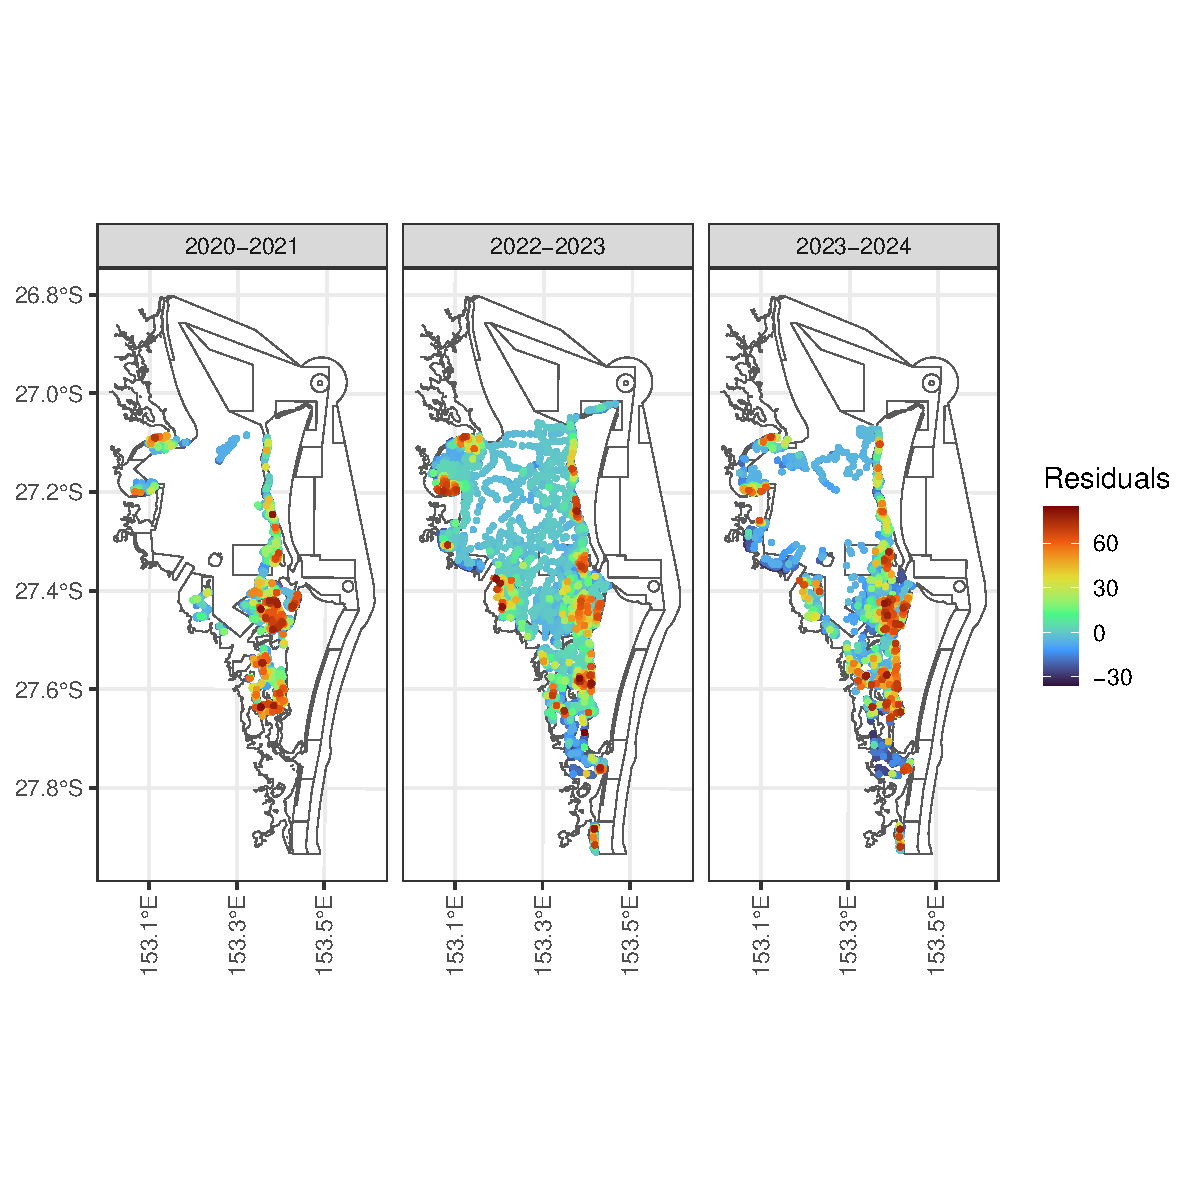
\includegraphics[keepaspectratio]{MBreport_files/figure-pdf/fig-resid_fy_mb-1.pdf}}

}

\caption{\label{fig-resid_fy_mb}Seagrass model residuals for resilience
analysis in Moreton Bay, by financial year.}

\end{figure}%

\begin{table}

\caption{\label{tbl-res_vars_mb}Covariates included in the resilience
model, including whether they were a fixed or random effect, and the
nonlinearity degree of the B-splines basis function.}

\centering{

\centering
\begin{tabular}{lll}
  \toprule
Variable & Effect & Degree \\ 
  \midrule
Coral Habitat Total Area & Fixed & 2 \\ 
  Seagrass Habitat Total Area & Fixed & 2 \\ 
  Mangrove Habitat Total Area & Fixed & 2 \\ 
  Gastropod Habitat Total Area & Fixed & 2 \\ 
  Distance to Coral Habitat & Fixed & 3 \\ 
  Distance to Seagrass Habitat & Fixed & 2 \\ 
  Distance to Mangrove Habitat & Fixed & 2 \\ 
  Distance to Gastropod Habitat & Fixed & 2 \\ 
  Species Richness & Fixed & 1 \\ 
  Habitat Count & Fixed & 2 \\ 
  Dominant Species & Fixed & NA \\ 
  Bathymetry Mean Depth & Fixed & 2 \\ 
  Bathymetry Mean Curvature & Fixed & 2 \\ 
  Bathymetry Mean Slope & Fixed & 2 \\ 
  EHMP Subzone & Random & NA \\ 
   \bottomrule
\end{tabular}

}

\end{table}%

\subsubsection{Statistical Modeling}\label{statistical-modeling}

\begin{table}

\caption{\label{tbl-mb-res-fixed}Fixed effects table of covariates in
the Moreton Bay resilience model.}

\centering{

\centering
\begin{tabular}{lrrr}
  \toprule
Term & Estimate & z & p.value \\ 
  \midrule
Intercept (Absent) & -30.413 & -2.588 & 0.010 \\ 
  CS & 47.680 & 32.519 & 0.000 \\ 
  HD & 6.182 & 1.071 & 0.284 \\ 
  HO & 12.965 & 14.788 & 0.000 \\ 
  HS & 20.025 & 21.705 & 0.000 \\ 
  SI & 19.904 & 4.908 & 0.000 \\ 
  ZMHU & 28.048 & 32.837 & 0.000 \\ 
  Species Richness & 1.911 & 4.710 & 0.000 \\ 
  Coral Area Deg1 & -8.420 & -1.620 & 0.105 \\ 
  Coral Area Deg2 & 1.939 & 0.272 & 0.786 \\ 
  Seagrass Area Deg 1 & -2.812 & -1.367 & 0.171 \\ 
  Seagrass Area Deg1 & -0.785 & -0.500 & 0.617 \\ 
  Mangrove Area Deg1 & -3.105 & -0.729 & 0.466 \\ 
  Mangrove Area Deg2 & 1.795 & 0.298 & 0.766 \\ 
  Gastropod Area Deg1 & 10.378 & 1.099 & 0.272 \\ 
  Gastropod Area Deg2 & -22.961 & -2.238 & 0.025 \\ 
  Habitat Count Deg1 & -1.428 & -0.488 & 0.625 \\ 
  Habitat Count Deg2 & 1.816 & 0.649 & 0.516 \\ 
  Coral Distance Deg1 & -5.043 & -0.615 & 0.539 \\ 
  Coral Distance Deg2 & 0.161 & 0.018 & 0.985 \\ 
  Coral Distance Deg3 & 0.999 & 0.131 & 0.895 \\ 
  Seagrass Distance Deg1 & 7.656 & 1.232 & 0.218 \\ 
  Seagrass Distance Deg2 & -11.543 & -1.110 & 0.267 \\ 
  Mangrove Distance Deg1 & -9.280 & -1.298 & 0.194 \\ 
  Mangrove Distance Deg2 & 7.514 & 0.918 & 0.359 \\ 
  Gastropod Distance Deg1 & 0.772 & 0.119 & 0.905 \\ 
  Gastropod Distance Deg2 & -3.009 & -0.749 & 0.454 \\ 
  Bathymetry Mean Depth Deg1 & 21.332 & 2.129 & 0.033 \\ 
  Bathymetry Mean Depth Deg2 & -2.460 & -0.374 & 0.708 \\ 
  Bathymetry Mean Slope Deg1 & 3.698 & 1.005 & 0.315 \\ 
  Bathymetry Mean Slope Deg2 & -9.865 & -1.930 & 0.054 \\ 
  Bathymetry Mean Curvature Deg1 & 16.126 & 1.398 & 0.162 \\ 
  Bathymetry Mean Curvature Deg2 & 23.319 & 2.568 & 0.010 \\ 
   \bottomrule
\end{tabular}

}

\end{table}%

Table~\ref{tbl-mb-res-fixed} shows the fixed effects table from the
fitted model. The reference group is the absent dominant species, and
the remaining dominant species terms represent deviations from this
baseline. Species richness, the only numeric variable with a single
level, had a large test statistic and small \(p\)-value (\(p\)-value
\(<\) 0.01). The other numeric variables were modeled using a B-spline
basis of at least degree two to capture nonlinearities. While we can
assess the overall significance of species richness in
Table~\ref{tbl-mb-res-fixed}, we must perform an analysis of variance
(ANOVA) to assess the overall significance the remaining variables with
multiple terms. Table~\ref{tbl-mb-res-anova} shows these ANOVA results.

\begin{table}

\caption{\label{tbl-mb-res-anova}ANOVA table of covariates in the
Moreton Bay resilience model.}

\centering{

\centering
\begin{tabular}{lrrr}
  \toprule
Effects & df & Chi-sq & p.value \\ 
  \midrule
Dominant Species &    6 & 1637.726 & 0.000 \\ 
  Bathymetry Mean Depth &    2 & 21.876 & 0.000 \\ 
  Bathymetry Mean Curvature &    2 & 8.999 & 0.011 \\ 
  Gastropod Habitat Total Area &    2 & 5.155 & 0.076 \\ 
  Bathymetry Mean Slope &    2 & 4.768 & 0.092 \\ 
  Coral Habitat Total Area &    2 & 2.845 & 0.241 \\ 
  Seagrass Habitat Total Area &    2 & 1.971 & 0.373 \\ 
  Distance to Mangrove Habitat &    2 & 1.871 & 0.392 \\ 
  Distance to Seagrass Habitat &    2 & 1.836 & 0.399 \\ 
  Habitat Count &    2 & 0.722 & 0.697 \\ 
  Distance to Gastropod Habitat &    2 & 0.613 & 0.736 \\ 
  Distance to Mangrove Habitat &    2 & 0.536 & 0.765 \\ 
  Distance to Coral Habitat &    3 & 0.718 & 0.869 \\ 
   \bottomrule
\end{tabular}

}

\end{table}%

We found strong evidence (\(p\)-value \textless{} 0.001) that dominant
species, species richness, and bathymetry mean depth are associated with
resilience:

\begin{itemize}
\tightlist
\item
  Dominant Species: The estimated (marginal) average resilience score is
  largest for CS (38.4), followed by ZMHU (18.8), HS (10.8), SI (10.7),
  HO (3.7), and HD (-3.1).
\item
  Species Richness: An increase of species richness by one species was
  associated with an average increase in resilience by approximately two
  units (Figure~\ref{fig-mb_res_rich_bath}).
\item
  Bathymetry Mean Depth: Deeper sites tended to be more resilient than
  shallower sites, on average (Figure~\ref{fig-mb_res_rich_bath}).
\end{itemize}

We found moderate evidence (\(p\)-value \textless{} 0.1) that bathymetry
mean curvature, gastropod habitat total area, and bathymetry mean slope
are associated with resilience:

\begin{itemize}
\tightlist
\item
  Bathymetry Mean Curvature: Sites with more curvature tended to be less
  resilient than sites with less curvature.
\item
  Gastropod Habitat Total Area: Sites with more gastropod habitat area
  tended to be more resilient than sites with less gastropod habitat
  area.
\item
  Bathymetry Mean Slope: Sites with less extreme slopes (between zero
  and one) tended to have increasing resilience with slope, while sites
  with more extreme slopes (greater than one) tended to have decreasing
  resilience with slope.
\end{itemize}

We found little evidence (\(p\)-value \textgreater{} 0.1) the remaining
variables were associated with resilience, after controlling for other
model covariates.

\begin{figure}

\centering{

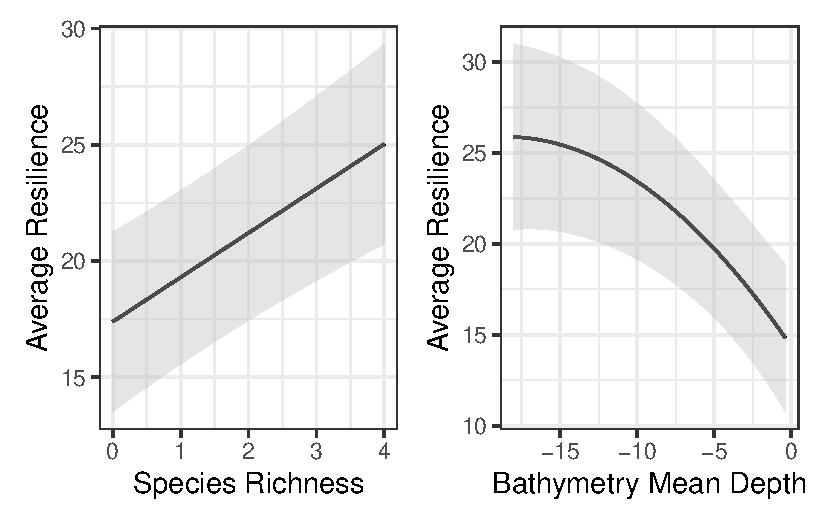
\includegraphics[width=0.8\linewidth,height=\textheight,keepaspectratio]{MBreport_files/figure-pdf/fig-mb_res_rich_bath-1.pdf}

}

\caption{\label{fig-mb_res_rich_bath}Average species richness (left) and
bathymetry mean depth (right) effects on resilience. Estimates (and
confidence intervals) were evaluated at the means of all other numeric
variables and for the ZMHU species in the Southern Bay.}

\end{figure}%

As mentioned previously, we also fit a random forest model to the
seagrass model residuals. Largely, the results were similar to the
spatial linear model. Notably, for the random forest:

\begin{itemize}
\tightlist
\item
  Dominant species was most important, with a similar ranking of
  resilient species as for the spatial linear model approach (e.g., CS,
  ZMHU most resilient and Absent least resilient).
\item
  Species richness was second-most important, with a general increasing
  trend in resilience with richness.
\item
  Distance to gastropod habitat was third-most important, with a
  decreasing trend at relatively short distances (\textless{} 15,000 m)
  and an increasing trend at large distances (\textgreater{} 15,000 m).
\item
  Bathymetry mean depth was the fourth-most important variable, with a
  general decreasing trend with decreasing depth
  (Figure~\ref{fig-rf_bathy}), which is similar to the spatial linear
  model results.
\item
  Seagrass area, distance to mangrove habitat, and distance to coral
  habitat had similar importance as the remaining bathymetry variables.
\item
  The remaining variables (distance to seagrass habitat, mangrove area,
  EHMP subzone, habitat count, coral area, and gastropod area) were
  least important.
\end{itemize}

The consistency between the two resilience models and their variable
importance rankings reinforce the spatial linear model's identification
of dominant species, species richness, and bathymetry mean depth as key
resilience drivers.

\begin{figure}

\centering{

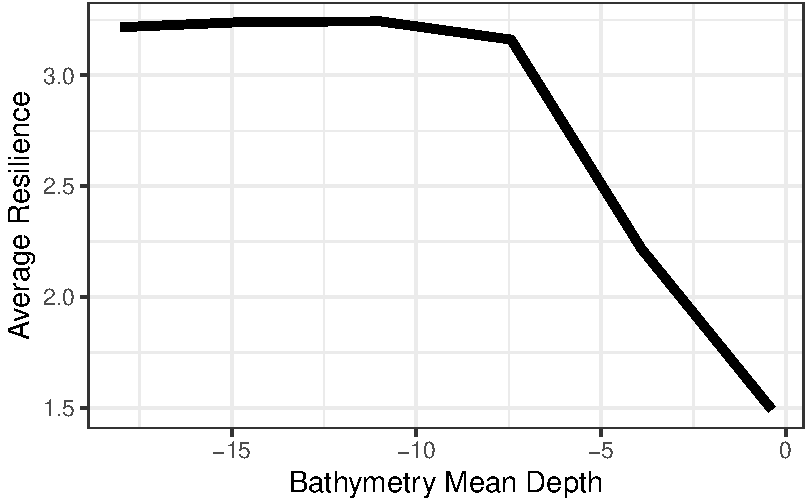
\includegraphics[width=0.5\linewidth,height=\textheight,keepaspectratio]{MBreport_files/figure-pdf/fig-rf_bathy-1.pdf}

}

\caption{\label{fig-rf_bathy}Random forest partial dependence for
resilience as a function of bathymetry mean depth.}

\end{figure}%

\section{Limitations}\label{limitations}

While the spatial linear model was useful for characterizing broad
patterns in seagrass cover related to tidal range, sediment type,
temperature, and turbidity and site-specific patterns capturing
resilience, all while accounting for spatial dependence, there are some
limitations. First, the eReefs water-quality covariates are based on
modeled data that are not directly observed in the field, potentially
propagating modeling error. Second, there are many correlated
water-quality variables, making it difficult for any model to isolate
the effects of each component of water quality pre- and post-flood.
Third, the lack of a covariate describing mean salinity in the 90 days
prior to sampling makes it challenging to directly study the effect of
mean salinity during the flood period. Fourth, seagrass cover data was
not collected in the first four months following the flood. It is
therefore unclear whether the seagrass data collected in the 2022-2023
financial year fully describe flood impacts. Fifth, covariates
representing local-scale drivers of seagrass cover (e.g., light
attenuation, biological interactions, etc.) were not available, which
might explain some additional variability in the response through space
and time. Sixth and finally, the location of sample sites was not
generated randomly and could be subject to conscious or unconscious
selection bias.

\section{Revisiting the Research
Questions}\label{revisiting-the-research-questions}

\textbf{Research Question 1}: Can we identify water quality covariates
that act as triggers for seagrass cover management responses? Are these
triggers different based on whether they result from a specific event
(e.g., flood) or are ambient?

We identified ambient 90-day turbidity, turbidity during the flood
event, and ambient 90-day water temperature as significant water quality
covariates in the seagrass cover model. Our results suggest that ambient
and flood-related turbidity act through distinct mechanisms and at
different magnitudes; a one-unit increase in 90-day mean turbidity was
associated with a 7.18 percentage point decrease in total cover, while
the effect of flood turbidity decayed with time since the flood. Across
tidal ranges, intertidal sites supported the highest average total cover
(26.89\%), followed by shallow subtidal (16.51\%) and deep subtidal
(4.88\%), suggesting that management thresholds may need to be
calibrated differently depending on depth zone. Similarly, sediment type
affected baseline cover levels, as sites with muddy sand and sandy mud
substrates supported higher average seagrass cover than sand or rock
sites. Together, these results suggest that management triggers should
differ depending on whether the driver is chronic ambient turbidity or
an acute flood event, and should further account for the tidal and
sediment context of the sites in question.

\textbf{Research Question 2}: Did seagrass cover improve after the flood
event(s)? If so, how and where?

Total seagrass cover improved throughout Moreton Bay between 2022--2023
and 2023--2024, suggesting the system has been recovering since the
flood. However, recovery was spatially heterogeneous; Deception Bay and
the Marine National Park zone returned to pre-flood cover levels, while
Southern Bay and the General Use Zone lagged considerably behind.
Recovery was also relatively slow compared to the magnitude of the
impact in the intertidal tidal range compared to shallow and deep
subtidal ranges, suggesting that intertidal sites may warrant
prioritized management attention immediately following floods.

\textbf{Research Question 3}: Can we identify site-specific resilience
indicators, which describe where recovery is likely to be enhanced or
impeded? What factors contribute to seagrass resilience?

We identified several site-specific indicators of seagrass resilience.
Dominant species, species richness, and bathymetry mean depth were the
strongest predictors of seagrass cover resilience, with sites dominated
by CS or ZMHU species, higher species richness, and greater water depth
tending to outperform model expectations and hence, infer greater
resilience. Gastropod habitat area, bathymetric curvature, and slope
provided moderate additional explanatory power. These findings may
suggest that deeper, species-rich meadows dominated by CS and ZMHU
exhibit a high level of resilience, while sites with low species
richness and/or dominated by other species may require more active
intervention to support recovery.

\section{Summary}\label{summary}

We applied a rigorous, spatially explicit statistical framework to
characterize the drivers, recovery, and resilience of seagrass cover in
Moreton Bay across a three-year monitoring period that included the 2022
Moreton Bay flood event. The analytical approach taken here is
well-suited to the structure and scale of the data, and the findings
have direct implications for adaptive management of the bay's seagrass
ecosystem.

The use of spatial linear models as the primary analytical framework is
well-justified from both statistical and ecological perspectives. Total
percent seagrass cover observations collected across the bay are
inherently spatially structured, as nearby sites share similar
environmental conditions, water quality and disturbance histories, as
well as ecological communities. Models that ignore this dependence may
well provide misleading results and inference. By explicitly modeling
spatial dependence via a spatial covariance function, the analyses
presented here produce more reliable estimates of covariate effects and
more honest characterizations of uncertainty than a conventional
non-spatial model provides. These models are typically also more
interpretable and characterize uncertainty more effectively than machine
learning models. The inclusion of EHMP subzone as a random effect
further accounts for structured variation among management-relevant
regions of the bay, ensuring that covariate estimates reflect
within-subzone patterns rather than being confounded by between-subzone
differences in baseline cover. The block Kriging helps understand
bay-wide trends and can immediately characterize bay-wide predictions on
the original total seagrass cover scale (0-100), rather than a
transformed scale required for generalized linear models; providing a
flexible framework for scenario modeling under future flood conditions
and climate scenarios.

The use of a two-stage modeling framework -- first modeling total
seagrass cover as a function of water quality and geographic drivers,
then modeling the seagrass model residuals as a function of site-level
resilience covariates -- is a structured approach to separating bay-wide
environmental patterns from site-specific ecological resilience
capacity. This builds directly on the framework proposed by
\citet{gilby2023drivers} to help understand drivers of average
resilience and provide useful insight needed to inform broader
conservation strategies. The robustness of the findings is further
supported by the general consistency of results across multiple modeling
approaches (e.g., spatial beta regression model, random forest, etc.),
which provides evidence that the relationships identified are genuine
rather than resulting solely from specific modeling frameworks.

Overall, the results described in this report provide a quantitative,
spatially structured foundation for adaptive decision making. Together,
the identification of important water quality and geographic variables,
bay-wide predictions via block Kriging, and the characterization of
site-level resilience indicators provide data-driven evidence that can
inform temporally targeted, context-specific interventions throughout
Moreton Bay.

\clearpage

\section*{References}\label{references}
\addcontentsline{toc}{section}{References}

\renewcommand{\bibsection}{}
\bibliography{references.bib}

\section{Acknowledgements}\label{acknowledgements}

The seagrass cover dataset was provided by Science Under Sail Australia
(SUSA; https://www.scienceundersail.com.au/). The eReefs datasets (model
simulations, satellite or in-situ observations) and software were
produced as part of the eReefs project (ereefs.org.au), which is a
collaboration between Australia's national science agency CSIRO, the
Australian Institute of Marine Science (AIMS) and the Queensland
Government, with observations obtained through the Integrated Marine
Observing System (IMOS) and the Great Barrier Reef Marine Park Authority
(GBRMPA). eReefs is funded by the Australian Government's Reef Trust.

\clearpage

\section*{Appendix 1. Spatial Linear Models and Random Forest
Models}\label{appendix-1.-spatial-linear-models-and-random-forest-models}
\addcontentsline{toc}{section}{Appendix 1. Spatial Linear Models and
Random Forest Models}

The spatially explicit statistical models (i.e., spatial models) we used
to answer these research questions are related to commonly used linear
and generalized linear models but incorporate \emph{spatial dependence}.
Spatial dependence measures how similar two sites are based on their
distance. Formally, we can build spatial dependence directly into
spatial models by leveraging Tobler's First Law of Geography
\citep{tobler1970computer}, which states succinctly that ``nearby sites
tend to be more similar than distant sites''. Not only is this intuitive
from a ``first principles'' perspective, but spatial models also provide
many advantages for modeling spatial data compared to models that assume
independence among observations (i.e., nonspatial models). First,
nonspatial models tend to underestimate uncertainty, yielding covariate
standard errors and p-values for covariates that are too small and
corresponding confidence intervals that are too narrow. Second, spatial
models improve prediction at unsampled locations by borrowing strength
from nearby observations, yielding more precise predictions and
corresponding standard errors that vary by location. Third, spatial
models decompose model error into separate spatial and nonspatial
components, informing residual and resilience structure in ways that
nonspatial models cannot. Fourth, spatial models can provide
ecologically meaningful insight into the spatial dependence structure of
the process, informing relationships among measured and unmeasured
variables as well as future sampling plans. \citet{zimmerman2024spatial}
provide a thorough review of spatial models for ecological and
environmental data, providing more detail and justification for the
claims made above.

Spatial models also offer many benefits over commonly used machine
learning algorithms like random forests
\citep{breiman2001random, cutler2007random, james2017introduction, kuhn2022tidy}.
First, traditional machine learning algorithms do not incorporate
spatial dependence and, by consequence, often perform worse than spatial
models at characterizing important covariates and predicting at
unobserved locations \citep{fox2020comparing}. Second, machine learning
algorithms struggle to quantify uncertainty in a principled manner,
something spatial models excel at. Third, covariate inference is more
straightforward using spatial models, as they naturally provide p-values
that enable structured testing of hypotheses. Fourth, spatial models
provide a rich set of diagnostics like leverage and Cook's distances
\citep{montgomery2021introduction}, quantities not generally defined for
machine learning algorithms. This is not to say that machine learning
algorithms cannot be very useful in ecological data analyses, but rather
that spatial models are sometimes a more effective tool for modeling
spatial data.

Though there are many benefits of spatial models over machine learning
algorithms, the reverse is also true. It is much simpler to capture
complex nonlinearities using ``out-of-the-box'' machine learning
algorithms, bypassing the tuning often required for spatial models that
involve nonlinear components like splines. This can be especially useful
for ecological data, which often exhibit nonlinear relationships
\citep{fox2017assessing}. Machine learning algorithms also typically
rely on few, if any, distributional assumptions and can be more robust
against unusual observations like outliers \citep{hastie2009elements}.
Machine learning algorithms also tend to be much more computational
efficient than spatial models. Importantly, machine learning algorithms
and spatial models can be complementary tools that help shed insight
into complicated ecological processes (something we reiterate in the
upcoming analyses). An exciting and developing area of statistical
research involves incorporating spatial modeling strategies directly
into machine learning algorithms
\citep{saha2023random, heaton2025scalable}.

The first spatially explicit model we define is the spatial linear
model. The spatial linear model is a \emph{mixed-effects model}
\citep{pinheiro2000mixed, bolker2015linear} written as

\begin{equation}\phantomsection\label{eq-splm1}{
y_i = \beta_0 + \beta_1x_{1, i} + \beta_2x_{2, i} + ... + \beta_p x_{p, i} + \tau_i + \epsilon_i,
}\end{equation} where \(i = 1, 2, ..., n\) indexes the \(n\)
observations. The quantity \(y_i\) is the response variable (for
observation \(i\)). The quantity \(\beta_j\) is a slope parameter that
controls the average effect of the covariate \(x_{j, i}\) on \(y_i\)
(while holding all other covariates constant). The random error
\(\tau_i\) is a spatial random error, and the random error
\(\epsilon_i\) is the nonspatial (i.e., independent) random error. The
spatial random error is spatially structured, capturing spatial residual
effects like environmental gradients we do not have data to fully
represent. The nonspatial random error is not spatially structured and
captures nonspatial residual effects like measurement error and
microscale variation. The difference between a traditional (i.e.,
nonspatial) linear model and a spatial linear model is the inclusion of
\(\tau_i\) (in the spatial linear model). The spatial random error
implied by \(\tau_i\) is governed by a \emph{spatial covariance
function}. The spatial covariance function allows the model to
incorporate spatial dependence, yielding the improved model performance
previously described. Figure~\ref{fig-spcov_fns} shows three different
spatial covariance functions that describe different ways the spatial
covariance decays with distance. Model parameters and standard errors
are estimated from data using likelihood-based
\citep{patterson1971recovery, harville1977maximum, wolfinger1994computing}
or semivariogram-based \citep{cressie1985fitting, curriero1999composite}
estimation methods. Often, the spatial linear model in
Equation~\ref{eq-splm1} is written more compactly using \emph{matrix
notation}: \begin{equation}\phantomsection\label{eq-splm2}{
\mathbf{y} = \mathbf{X} \boldsymbol{\beta} + \boldsymbol{\tau} + \boldsymbol{\epsilon},
}\end{equation} where \(\mathbf{X}\) is a matrix that holds the \(j\)
covariates for each of \(n\) observations, and \(\mathbf{y}\),
\(\boldsymbol{\beta}\), \(\boldsymbol{\tau}\), and
\(\boldsymbol{\epsilon}\) are vectors that contain each of the \(n\) or
\(j\) quantities from Equation~\ref{eq-splm1}. The spatial linear model
can be adjusted to account for nonspatial random effects just as one
would add random effects to a nonspatial linear mixed model:
\begin{equation}\phantomsection\label{eq-splm3}{
\mathbf{y} = \mathbf{X} \boldsymbol{\beta} + \mathbf{Z}\mathbf{u} + \boldsymbol{\tau} + \boldsymbol{\epsilon},
}\end{equation} where \(\mathbf{Z}\) is a random effect design matrix
(dimension \(n \times k\)) that indexes each of the \(k\) random effects
in \(\mathbf{u}\). For more information about specific forms of various
spatial covariance functions, see \citet{schabenberger2017statistical}
and \citet{zimmerman2024spatial}.

\begin{figure}

\centering{

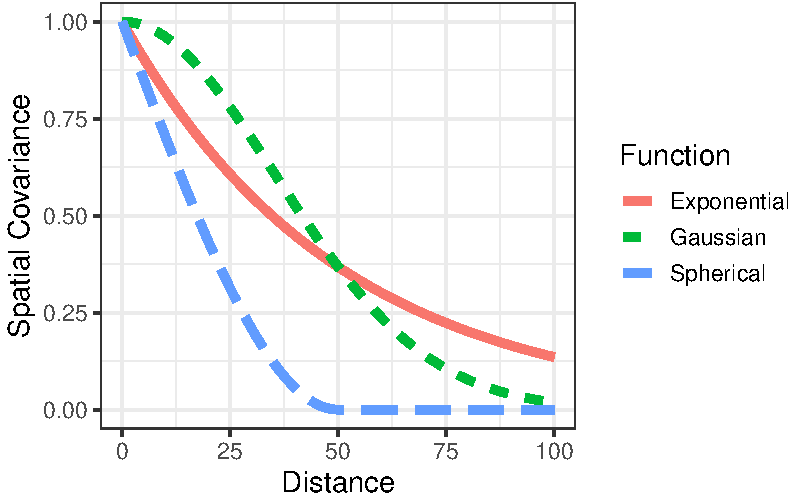
\includegraphics[width=0.75\linewidth,height=\textheight,keepaspectratio]{MBreport_files/figure-pdf/fig-spcov_fns-1.pdf}

}

\caption{\label{fig-spcov_fns}Three spatial covariance functions that
represent different spatial dependence behavior.}

\end{figure}%

Like the traditional linear model, the spatial linear model can capture
complex nonlinearities in the data through the use of interaction
effects \citep{faraway2002practical, lenth2025emmeans}, splines
\citep{chambers1992statistical, ruppert2003semiparametric}, additive
models \citep{wood2017generalized, pedersen2019hierarchical}, and
penalized regression models like the ridge and lasso
\citep{tibshirani1996regression}. Generally, this is accomplished by
leveraging \emph{basis functions} that break down nonlinear behavior
into a set of additive linear components that may include penalty terms
which guard against overfitting. Furthermore, there is no assumption
that \(y_i\) itself is normally distributed; rather, distributional
assumptions are placed on the random errors after incorporating the
slope parameters. This clarification implies the spatial (and
nonspatial) linear models can be quite effective at modeling a range of
data that are not normally distributed. For highly nonnormal data, tools
like generalized linear models, which we discuss later, can be helpful.
Finally, under general conditions, the slope parameters of the spatial
(and nonspatial) linear models are approximately normally distributed
with a large sample size (see \citet{casella2024statistical} for a
general justification via the Central Limit Theorem and
\citet{zhang2005towards} for nuances regarding spatial data). This is
beneficial because it justifies valid hypothesis testing on the slope
coefficients (often of primary ecological interest), no matter the
distribution of the data (given certain assumptions are satisfied).

One of the most useful applications of the spatial linear model is
predicting the response variable at unobserved locations. A very useful
spatial prediction method called Kriging has a rich theoretical
justification \citep{cressie1990origins, stein1999interpolation}.
Kriging is the spatial analogue to best linear unbiased prediction
(BLUP) for mixed models \citep{henderson1975best}. Via Kriging, the
spatial linear model produces BLUPs at each unobserved location of
interest, alongside prediction intervals to characterize uncertainty.
While useful, sometimes the goal is to create a BLUP for an entire
region of interest based on realized (i.e., observed) covariate values.
This technique, which builds upon the theoretical foundations of
Kriging, is called block Kriging
\citep{ver2002sampling, cressie2006block}. The intuition is to make
point predictions at a very dense grid in the study region and then
average these predictions, appropriately characterizing uncertainty.
Together, Kriging and block Kriging provide a complete set of tools for
spatial prediction, given the fit of a spatial linear model.

Spatial generalized linear models are an extension of spatial linear
models to highly nonnormal data
\citep{christensen2002bayesian, zhang2002estimation, diggle2007model, bonat2016practical}.
\citet{verhoef2024marginal} proposed a novel application of the Laplace
approximation to enable restricted maximum likelihood estimation of
spatial generalized linear models. This model formulation builds upon
Equation~\ref{eq-splm1} and is given by
\begin{equation}\phantomsection\label{eq-spglm1}{
g(\mu_i) = \beta_0 + \beta_1x_{1, i} + \beta_2x_{2, i} + ... + \beta_p x_{p, i} + \tau_i + \epsilon_i,
}\end{equation} where \(g(\mu_i)\) is a ``link function'' that links the
distribution of \(y_i\) to a linear function of its mean, \(\mu_i\).
Common link functions include the log link for count and skewed data and
the logit link for binomial and proportion data
(Table~\ref{tbl-glm-families}). Using the same argument as for spatial
linear models, nonspatial random effects can be added to spatial
generalized linear models.

\begin{table}

\caption{\label{tbl-glm-families}Common generalized linear model
families, link functions, and appropriate data types.}

\centering{

\centering
\begin{tabular}{llll}
  \toprule
Family & Link Function & Link Name & Data Type \\ 
  \midrule
Binomial & $f(\mu) = \log(\mu / (1 - \mu))$ & Logit & Binary; Binary Count \\ 
  Poisson & $f(\mu) = \log(\mu)$ & Log & Count \\ 
  Negative Binomial & $f(\mu) = \log(\mu)$ & Log & Count \\ 
  Beta & $f(\mu) = \log(\mu / (1 - \mu))$ & Logit & Proportion \\ 
  Gamma & $f(\mu) = \log(\mu)$ & Log & Skewed \\ 
  Inverse Gaussian & $f(\mu) = \log(\mu)$ & Log & Skewed \\ 
   \bottomrule
\end{tabular}

}

\end{table}%

Spatial models are complicated, both theoretically and computationally.
This has contributed to their relative underuse in the ecological
community. However, recent advances in open-source software have made
spatial models more accessible to ecologists who have strong subject
matter expertise but may lack sufficient statistical background or
computational skills to implement them from scratch. One such
advancement is the \texttt{spmodel} \textbf{R} package
\citep{dumelle2023spmodel}, which emulates base-\textbf{R} functions
like \texttt{lm()} and \texttt{glm()} to account for spatial dependence
via \texttt{splm()} and \texttt{spglm()}, respectively. Familiar
\textbf{R} functions like \texttt{summary()} and \texttt{predict()} can
be used directly on models fit via \texttt{spmodel}. Importantly,
\texttt{spmodel} also has tools for spatial random forest residual
modeling \citep{fox2020comparing}, applications to large data of several
thousand observations via spatial indexing \citep{ver2023indexing}, and
cross validation \citep{stone1974cross, roberts2017cross}.





\end{document}
